% Part 1: qmd image positions 07-45. Content from old slide P-1, qualified by the lecture prose.
\tikzset{el/.style={draw=#1, thick, fill=#1!12, minimum width=0.85cm, minimum height=0.85cm, rounded corners=2pt}}

% pos 07
\begin{frame}{Seaweeds take up nutrients across the whole thallus}
\twocol{
\begin{itemize}
  \item Algae, like land plants, need nutrients for persistence, growth and reproduction
  \item Seaweeds are bathed in the medium that supplies them (intertidal species for most of the time)
  \item Uptake occurs across the thallus surface: no roots are needed
  \item Surface area to volume ratio therefore matters (Lecture 2)
  \item Many land plants rely on mycorrhizae or root nodules; seaweeds have their own uptake systems
\end{itemize}}{
\begin{tikzpicture}[font=\scriptsize]
  \fill[sea!12] (-3.6,-1.2) rectangle (-0.3,2.6);
  \node[font=\scriptsize\bfseries, sea] at (-1.95,2.3) {Seaweed};
  \draw[leaf, line width=5pt, line cap=round] (-1.95,-1.0) .. controls (-2.4,0.4) and (-1.4,1.0) .. (-1.9,2.0);
  \draw[leaf, line width=3pt, line cap=round] (-2.0,0.4) .. controls (-2.8,0.9) .. (-3.0,1.6);
  \draw[leaf, line width=3pt, line cap=round] (-1.8,0.8) .. controls (-1.0,1.2) .. (-0.8,1.8);
  \foreach \x/\y in {-3.2/-0.5,-2.8/0.2,-1.1/0.3,-0.7/-0.6,-2.5/1.9,-1.2/2.0,-3.3/1.1,-0.9/1.1}
    \node[font=\scriptsize, sea] at (\x,\y) {N};
  \fill[warm!25] (0.3,-1.2) rectangle (3.6,0.5);
  \fill[sea!8] (0.3,0.5) rectangle (3.6,2.6);
  \node[font=\scriptsize\bfseries, warm] at (1.95,2.3) {Land plant};
  \draw[leaf, line width=3pt] (1.95,0.5) -- (1.95,1.9);
  \fill[leaf] (1.95,1.9) ellipse (0.5 and 0.25);
  \draw[warm!70!black, thick] (1.95,0.5) -- (1.6,-0.4) -- (1.2,-0.9) (1.95,0.5) -- (2.3,-0.3) -- (2.9,-0.8) (1.95,0.5) -- (1.95,-1.0);
  \foreach \x/\y in {0.7/-0.3,1.0/-1.0,2.6/-0.5,3.2/-0.2,2.2/-1.0}
    \node[font=\scriptsize, warm!70!black] at (\x,\y) {N};
  \node[font=\scriptsize, align=center, text width=3.1cm] at (-1.95,-1.65) {uptake over the whole surface};
  \node[font=\scriptsize, align=center, text width=3.1cm] at (1.95,-1.65) {uptake through roots, often with symbionts};
\end{tikzpicture}
\fignote{Schematic.}}
\end{frame}

% pos 08
\begin{frame}{Essential and beneficial nutrients}
\twocol{
\begin{itemize}
  \item Much of what we know about algal nutrition comes from work on culture media between the 1930s and 1970s
  \item These studies identified \textbf{essential} and \textbf{beneficial} nutrients
  \item Beneficial nutrients promote growth or function but are not required to complete the life cycle
\end{itemize}}{
\begin{tikzpicture}[font=\scriptsize]
  \node[card=accent, text width=6.4cm] (e) {\textbf{Essential} (Epstein 1972): either criterion is sufficient\\[4pt]
    1. the plant cannot complete a normal life cycle without it; or\\[2pt]
    2. it is part of an essential constituent or metabolite, e.g.\ Mg in chlorophyll-\textit{a}};
  \node[card=sand, text width=6.4cm, below=0.5cm of e] {\textbf{Beneficial}\\[4pt] enhances growth or a physiological process in some species, without being strictly required};
\end{tikzpicture}}
\end{frame}

% pos 09
\begin{frame}{A second test of essentiality}
\twocol{
\begin{itemize}
  \item An alternative definition sets three conditions
  \item The first overlaps with Epstein's life-cycle criterion
  \item An essential role may be structural, metabolic or as an enzyme cofactor
\end{itemize}}{
\begin{tikzpicture}[font=\scriptsize]
  \node[flow=hot, text width=6.0cm] (a) {\textbf{1. Growth fails}\\ when the element is lacking};
  \node[flow=warm, text width=6.0cm, below=0.35cm of a] (b) {\textbf{2. It cannot be replaced}\\ no other element performs the same function};
  \node[flow=accent, text width=6.0cm, below=0.35cm of b] (c) {\textbf{3. Its effect is direct}\\ it acts in metabolism itself, not only through an interaction with another factor};
\end{tikzpicture}}
\end{frame}

% pos 10
\begin{frame}{Macronutrients and micronutrients}
\twocol{
\begin{itemize}
  \item Classified by the quantity in tissue or the amount needed in nutrient solutions
  \item Quantity says nothing about importance: every essential element is required
  \item Macronutrients: mainly structural; some are also regulatory (e.g.\ Ca, Mg)
  \item Micronutrients: catalytic and regulatory
\end{itemize}}{
\begin{tikzpicture}[font=\scriptsize]
  \node[card=sea, text width=2.9cm, minimum height=3.6cm, anchor=north] at (-1.7,0) {\textbf{Macro}\\[3pt] C, H, O, N, P, K, Ca, Mg, S\\[4pt] build biomass: proteins, nucleic acids, membranes, walls};
  \node[card=warm, text width=2.9cm, minimum height=3.6cm, anchor=north] at (1.7,0) {\textbf{Micro}\\[3pt] Fe, Mn, Zn, Cu, Mo, B, Cl, Ni \ldots\\[4pt] enzyme cofactors, e.g.\ Fe and Mo in nitrate reductase};
\end{tikzpicture}
\fignote{Lists after Lobban and Harrison (1997, Table 5.2) and Hopkins and Hüner (2008, Table 4.4).}}
\end{frame}

% pos 11
\begin{frame}{About twenty elements are needed by algae}
\twocol{
\begin{itemize}
  \item Around 20 elements support critical metabolic pathways in algae
  \item Algae and land plants share most of them; amounts differ
  \item Some are needed only by certain groups (e.g.\ Si in diatoms)
\end{itemize}}{
\begin{tikzpicture}[font=\scriptsize]
  \foreach \e [count=\i from 0] in {C,H,O,N,P,K,Ca,Mg,S}
    \node[el=sea] at ({mod(\i,5)*1.0},{-floor(\i/5)*1.0}) {\e};
  \foreach \e [count=\i from 0] in {Fe,Mn,Zn,Cu,Mo,B,Cl,Co,Na,Br,I}
    \node[el=warm] at ({mod(\i,5)*1.0},{-2.4-floor(\i/5)*1.0}) {\e};
  \node[font=\scriptsize\bfseries, sea, anchor=west] at (-0.45,0.75) {macronutrients};
  \node[font=\scriptsize\bfseries, warm, anchor=west] at (-0.45,-1.65) {micronutrients and elements needed by some seaweeds};
\end{tikzpicture}
\fignote{See Lobban and Harrison (1997, Table 5.1) for the elements and their functions.}}
\end{frame}

% pos 12
\begin{frame}{Functions of essential elements in seaweeds}
\centering\scriptsize
\renewcommand{\arraystretch}{0.9}
\begin{tabular}{@{}>{\bfseries}l>{\raggedright\arraybackslash}p{5.9cm}>{\raggedright\arraybackslash}p{6.1cm}@{}}
Element & Probable functions & Examples of compounds\\\hline
N & major metabolic importance in compounds & amino acids, purines, pyrimidines, amino sugars, amines\\
P & structural, energy transfer & ATP, GTP, nucleic acids, phospholipids, coenzyme A\\
K & osmotic regulation, pH control, protein conformation & occurs mainly in ionic form\\
Ca & structural, enzyme activation, ion transport & calcium alginate, calcium carbonate\\
Mg & photosynthetic pigments, enzyme activation, ribosome stability & chlorophyll\\
S & active groups in enzymes and coenzymes, structural & cystine, glutathione, agar, carrageenan, sulfolipids\\
Fe & porphyrin molecules and enzymes & ferredoxin, cytochromes, nitrate reductase\\
Mn & electron transport in photosystem II & \\
Cu & electron transport in photosynthesis, enzymes & plastocyanin, amine oxidase\\
Zn & enzymes & carbonic anhydrase\\
Mo & nitrate reduction, ion absorption & nitrate reductase\\
Co & component of vitamin B$_{12}$ & B$_{12}$\\\hline
\end{tabular}
\fignote{After DeBoer (1981), in Lobban and Harrison (1997, Table 5.1). Selected rows.}
\end{frame}

% pos 13
\begin{frame}{Tissue concentrations in land plants}
\centering
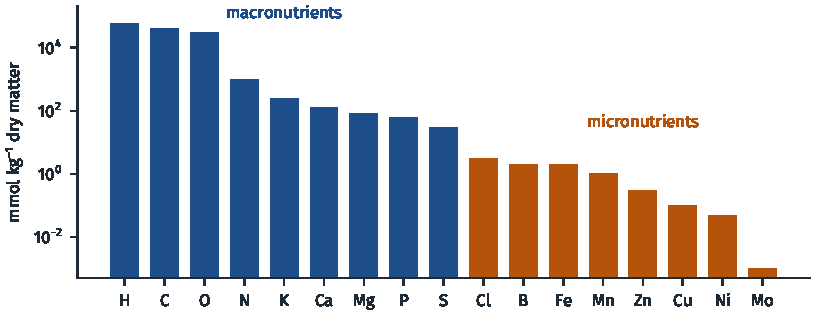
\includegraphics[width=0.86\textwidth]{fig_plant_tissue}
\fignote{Concentrations in dry matter considered adequate for normal growth of higher plants (Epstein 1972; Hopkins and Hüner 2008, Table 4.4). Logarithmic axis: macronutrients exceed micronutrients by several orders of magnitude.}
\end{frame}

% pos 14
\begin{frame}{Tissue and seawater concentrations}
\twocol{
\begin{itemize}
  \item C, H, O, N and P make up the bulk of algal dry matter
  \item Micronutrients and vitamins occur in much smaller amounts and rarely limit growth to the same extent
  \item N and P are about 100,000 times, and C about 10,000 times, more concentrated in the thallus than in seawater
  \item Much of tissue N is organic: compare the same dissolved form on both sides of the membrane
\end{itemize}}{
\begin{tikzpicture}[font=\scriptsize]
  \node[flow=sea, text width=2.4cm, minimum height=1.4cm] (w) at (-2.1,0) {\textbf{Seawater}\\ dissolved N, µM};
  \node[flow=leaf, text width=2.4cm, minimum height=1.4cm] (t) at (2.1,0) {\textbf{Thallus}\\ total N, mostly organic};
  \draw[arr] (w) -- node[above, font=\scriptsize] {uptake} (t);
  \node[card=grey, text width=6.0cm, font=\scriptsize] at (0,-2.2) {Whether transport is uphill depends on the \textbf{electrochemical gradient} of the free dissolved ion: concentration and membrane voltage. Total tissue N cannot show this.};
\end{tikzpicture}
\fignote{Concentration factors from Lobban and Harrison (1997, Table 5.2).}}
\end{frame}

% pos 15
\begin{frame}{Vitamins and organic nutrients}
\twocol{
\begin{itemize}
  \item Many algae also require \textbf{vitamins}: mainly B$_{12}$, thiamine and biotin
  \item These are often added to culture media to promote growth
  \item Some algae use \textbf{dissolved organic compounds}: amino acids as an N source, acetate as a C source
  \item Such mixotrophy is less common and is not the focus of this lecture
\end{itemize}}{
\begin{tikzpicture}[font=\scriptsize]
  \node[flow=leaf, minimum width=2.6cm, minimum height=1.2cm] (a) at (0,0) {\textbf{Alga}};
  \node[flow=sea, text width=2.6cm] (i) at (-2.3,1.6) {inorganic ions\\ NO$_3^-$, NH$_4^+$, PO$_4^{3-}$};
  \node[flow=warm, text width=2.6cm] (v) at (2.3,1.6) {vitamins\\ B$_{12}$, thiamine, biotin};
  \node[flow=accent, text width=2.6cm] (o) at (0,-2.0) {organic compounds\\ amino acids, acetate};
  \draw[arr] (i) -- (a); \draw[arr] (v) -- (a); \draw[arr] (o) -- (a);
\end{tikzpicture}
\fignote{Schematic.}}
\end{frame}

% pos 16
\begin{frame}{Elements are concentrated in seaweed tissue}
\twocol{
\begin{itemize}
  \item Ratio of mean concentration in seaweed dry matter to that in seawater
  \item N and P (red) are among the most concentrated macronutrients
  \item Trace metals such as Fe and Mn are scarce in seawater, so their ratios are very large
  \item Tissue values include organic and stored forms
\end{itemize}}{
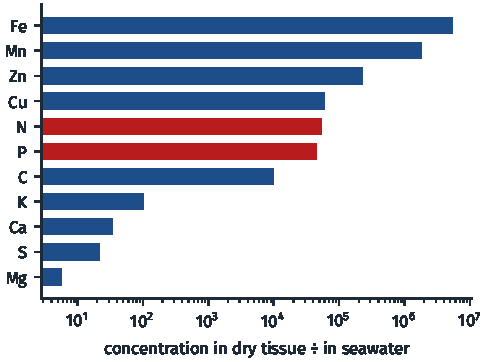
\includegraphics[width=\linewidth]{fig_concentration_factor}
\fignote{Calculated from DeBoer (1981), in Lobban and Harrison (1997, Table 5.2); logarithmic axis.}}
\end{frame}

% pos 17
\begin{frame}{Testing for a limiting nutrient}
\twocol{
\begin{itemize}
  \item Early work identified N as the nutrient most often limiting algal growth in the sea (Dugdale 1967)
  \item Adding N to seaweed aquaculture can greatly increase growth
  \item In some systems P limits, and P addition has similar effects
  \item Test with additions: control, +N, +P, +N+P, other conditions matched
  \item A null response to one nutrient leaves its role open: another factor may also restrict growth
\end{itemize}}{
\begin{tikzpicture}[font=\scriptsize]
\begin{axis}[ybar, width=7.6cm, height=5.4cm, bar width=0.9cm, ymin=0, ymax=1.15,
  symbolic x coords={control,+P,+N,+N+P}, xtick=data, ytick=\empty, axis lines=left,
  ylabel={\footnotesize growth response}, x tick label style={font=\scriptsize}, enlarge x limits=0.18, clip=false]
  \addplot[fill=sea!60, draw=sea] coordinates {(control,0.25) (+P,0.27) (+N,0.6) (+N+P,1.0)};
\end{axis}
\end{tikzpicture}
\fignote{Schematic outcome for an alga primarily limited by N, with P limiting once N is added.}}
\end{frame}

% pos 18
\begin{frame}{The Redfield ratio}
\twocol{
\begin{itemize}
  \item Microalgae and seaweeds differ in the relative amounts of C, N and P
  \item Marine plankton: C:N:P about 106:16:1, the \textbf{Redfield ratio} (Redfield 1958)
  \item Benthic marine plants: about 550:30:1 (Atkinson and Smith 1983)
  \item Seaweeds hold much more C per P: structural carbon and storage polysaccharides
  \item These are empirical summaries; composition varies with species and conditions
\end{itemize}}{
\begin{tikzpicture}[font=\scriptsize]
  \node[font=\scriptsize\bfseries] at (1.6,3.6) {atoms per atom of P};
  \foreach \lab/\c/\n/\y/\col in {plankton/106/16/2.4/sea, benthic plants/550/30/0.6/leaf}{
    \node[anchor=east, font=\scriptsize] at (-0.1,\y) {\lab};
    \fill[\col!70] (0,\y-0.2) rectangle ({\c/550*3.4},\y+0.2);
    \node[anchor=west, font=\scriptsize] at ({\c/550*3.4+0.05},\y) {C \c};
    \fill[\col!40] (0,\y-0.65) rectangle ({\n/550*3.4*6},\y-0.35);
    \node[anchor=west, font=\scriptsize] at ({\n/550*3.4*6+0.05},\y-0.5) {N \n\ (bar $\times$6)};
  }
\end{tikzpicture}
\fignote{N bars drawn six times longer than the C scale so that they remain visible.}}
\end{frame}

% pos 19
\begin{frame}{Which ratio answers which question?}
\twocol{
\begin{itemize}
  \item Reported optimal N:P ratios for seaweed cultivation vary widely (ca.\ 10:1 to 80:1)
  \item Ratios guide fertilising strategies in tank culture and predictions about eutrophication
  \item A deviation from a reference ratio suggests a hypothesis about nutrient status
  \item Test it with nutrient additions, tissue measurements and the growth response
\end{itemize}}{
\begin{tikzpicture}[font=\scriptsize]
  \node[card=leaf, text width=6.0cm] (a) {\textbf{Tissue composition}: what the alga contains, including stores};
  \node[card=sea, text width=6.0cm, below=0.3cm of a] (b) {\textbf{Dissolved concentration}: what is in the water now};
  \node[card=warm, text width=6.0cm, below=0.3cm of b] (c) {\textbf{Supply rate}: how fast N and P are delivered and renewed};
  \node[font=\scriptsize, grey, below=0.25cm of c, text width=6cm, align=center] {Keep these separate before comparing ratios};
\end{tikzpicture}}
\end{frame}

% pos 20
\begin{frame}{Liebig's law of the minimum}
\twocol{
\begin{itemize}
  \item Justus von Liebig (1803--1873) studied the chemistry of fertilisers
  \item If one essential nutrient is deficient, growth is poor even when all others are plentiful
  \item Supplying the deficient element increases growth until it no longer limits
  \item Beyond that point another resource is in shortest supply and limits instead
\end{itemize}}{
\begin{tikzpicture}[font=\scriptsize]
  \foreach \lab/\hh/\c [count=\i from 0] in {light/3.6/sand!55, K/3.3/sand!55, P/1.6/hot!45, N/3.8/sand!55, Fe/3.0/sand!55, CO$_2$/3.5/sand!55}{
    \fill[\c, draw=warm!70!black] (\i*0.62,0) rectangle (\i*0.62+0.56,\hh);
    \node[rotate=90, anchor=west] at (\i*0.62+0.28,0.1) {\lab};
  }
  \fill[sea!35, opacity=0.6] (0,0) rectangle (3.66,1.6);
  \draw[sea, very thick] (0,1.6) -- (3.66,1.6);
  \node[sea, anchor=west, font=\scriptsize] at (3.8,1.6) {attainable growth};
  \draw[-{Stealth}, hot, thick] (4.6,0.9) -- (1.9,1.25);
  \node[hot, anchor=west, font=\scriptsize] at (4.6,0.8) {shortest stave};
\end{tikzpicture}
\fignote{Schematic: the stave barrel. Water rises only to the shortest stave.}}
\end{frame}

% pos 21
\begin{frame}{Limitation reflects requirement and supply}
\twocol{
\begin{itemize}
  \item Ambient concentration reflects the balance between the alga's requirement and the rate of supply
  \item Physical conditions and traits of the alga also restrict growth
  \item Several factors can restrict growth at once, or one after another
\end{itemize}}{
\begin{tikzpicture}[font=\scriptsize]
  \node[flow=leaf, minimum width=2.4cm, minimum height=1.1cm] (g) at (0,0) {\textbf{growth}};
  \foreach \t/\a/\c in {light intensity/90/sand, temperature/30/hot, water motion and boundary layer/-30/sea, algal density and self-shading/-90/accent, population and genetic capacity/-150/warm, nutrient supply/150/leaf}{
    \node[flow=\c, text width=2.3cm, font=\scriptsize] (n\a) at (\a:2.55) {\t};
    \draw[arr] (n\a) -- (g);
  }
\end{tikzpicture}
\fignote{Schematic.}}
\end{frame}

% pos 22
\begin{frame}{Accounting with the minimum model}
\twocol{
\begin{itemize}
  \item Suppose each new biomass unit needs 10 µmol N and 1 µmol P
  \item With 20 µmol N and 1 µmol P: P permits one unit; 10 µmol N remain unused
  \item Add 1 µmol P: the same N supports two units
  \item Beyond 2 µmol P, N limits
  \item Illustrative requirements, not a universal seaweed ratio
\end{itemize}}{
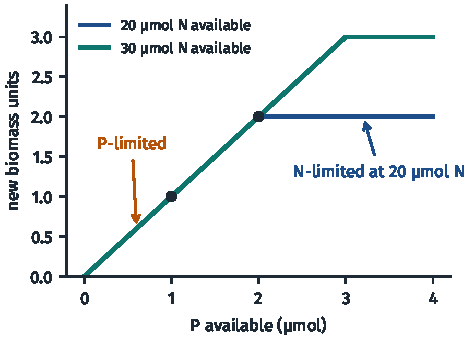
\includegraphics[width=\linewidth]{fig_liebig}
\fignote{Attainable biomass = min(N/10, P/1). Real responses involve reserves, variable composition and other constraints.}}
\end{frame}

% pos 23
\begin{frame}{Luxury consumption}
\twocol{
\begin{itemize}
  \item Uptake of more N or P than growth needs at the time
  \item The excess may remain in the medium, be stored as inorganic N or P in vacuoles, or be assimilated into organic compounds
  \item Stores are mobilised for growth when external supply declines
  \item An advantage where supply fluctuates; also used as a fertilising strategy in aquaculture
\end{itemize}}{
\begin{tikzpicture}[font=\scriptsize]
  \draw[arr] (0,0) -- (6.6,0) node[below left, ink] {time};
  \fill[sea!25] (0.6,0) rectangle (1.6,3.6);
  \node[sea, font=\scriptsize] at (1.1,3.85) {N pulse};
  \draw[very thick, sea] (0.2,0.3) -- (0.6,0.3) -- (0.6,3.4) -- (1.6,3.4) -- (1.6,0.2) -- (6.3,0.2);
  \draw[very thick, warm] (0.2,0.7) -- (0.6,0.7) .. controls (1.0,2.4) .. (1.6,2.6) .. controls (3.5,2.2) and (4.8,0.9) .. (6.3,0.7);
  \draw[very thick, leaf] (0.2,0.5) .. controls (3,1.6) and (4.5,2.6) .. (6.3,3.0);
  \node[sea, anchor=west, font=\scriptsize] at (4.4,0.45) {external N};
  \node[warm, anchor=west, font=\scriptsize] at (2.0,3.0) {internal reserve};
  \node[leaf, anchor=east, font=\scriptsize] at (6.3,3.4) {structural biomass};
\end{tikzpicture}
\fignote{Schematic. Uptake and growth occur at different times; storage capacity varies among species, tissues and conditions.}}
\end{frame}

% pos 24
\begin{frame}{Nitrogen as the worked example}
\twocol{
\begin{itemize}
  \item N most often limits algal growth in the sea
  \item N pollution drives eutrophication
  \item Uptake and assimilation of other nutrients follow similar principles
  \item Most concepts apply to both macroalgae and microalgae
\end{itemize}}{
\begin{tikzpicture}[font=\scriptsize]
  \node[flow=sea, text width=5.4cm] (a) {\textbf{Supply}: sources, cycling, concentrations};
  \node[flow=accent, text width=5.4cm, below=0.4cm of a] (b) {\textbf{Delivery}: water movement and the boundary layer};
  \node[flow=leaf, text width=5.4cm, below=0.4cm of b] (c) {\textbf{Uptake}: kinetics and membrane transport};
  \node[flow=hot, text width=5.4cm, below=0.4cm of c] (d) {\textbf{Consequences}: blooms and eutrophication};
  \draw[arr] (a) -- (b); \draw[arr] (b) -- (c); \draw[arr] (c) -- (d);
\end{tikzpicture}
\fignote{The route this lecture follows.}}
\end{frame}

% pos 26
\begin{frame}{Sources of nitrogen in the sea}
\twocol{
\begin{itemize}
  \item N$_2$ gas: about 78\% of the atmosphere; dissolved N$_2$ remains N$_2$ until fixed
  \item Biological N fixation converts N$_2$ to forms available to the food web
  \item Rivers, wastewater and atmospheric deposition bring reactive N to coastal waters
  \item Recycling within the ocean is of major importance
  \item Upwelling moves existing nutrient-rich water upwards
\end{itemize}}{
\begin{tikzpicture}[font=\scriptsize]
  \fill[sea!15] (-3.75,-2.6) rectangle (3.75,0.5);
  \node[sea, font=\scriptsize\bfseries, anchor=south west] at (-3.7,-2.55) {coastal ocean};
  \node[flow=grey, text width=2.0cm] (atm) at (-2.55,2.0) {atmosphere\\ N$_2$, NO$_x$};
  \node[flow=warm, text width=2.0cm] (riv) at (0,2.0) {rivers,\\ wastewater};
  \node[flow=hot, text width=2.0cm] (out) at (2.55,2.0) {losses to air\\ N$_2$, N$_2$O};
  \node[flow=leaf, text width=2.0cm] (fix) at (-2.55,-0.5) {N fixation\\ N$_2\rightarrow$ NH$_3$};
  \node[flow=sea, text width=2.6cm] (din) at (1.0,-0.5) {DIN pools\\ NO$_3^-$, NO$_2^-$, NH$_4^+$};
  \node[flow=accent, text width=2.2cm] (up) at (1.0,-1.95) {upwelling};
  \draw[arr] (atm) -- (fix); \draw[arr] (atm.south east) -- (din.north west);
  \draw[arr] (riv) -- (din); \draw[arr] (din) -- (out);
  \draw[arr] (fix) -- (din); \draw[arr] (up) -- (din);
\end{tikzpicture}
\fignote{Schematic. Pool sizes vary with depth, oxygen, biological activity and place.}}
\end{frame}

% pos 27
\begin{frame}{Fixation and transformations of nitrogen}
\twocol{
\begin{itemize}
  \item N-fixing microorganisms, including some cyanobacteria, reduce N$_2$ to ammonia
  \item Most photoautotrophs use nitrate, nitrite and ammonium
  \item \textbf{DIN} = NO$_3^-$ + NO$_2^-$ + NH$_4^+$, as N; it excludes dissolved N$_2$
  \item Nitrite is an intermediate; it accumulates where production exceeds consumption
\end{itemize}}{
\begin{tikzpicture}[font=\scriptsize, node distance=1.0cm]
  \node[flow=grey] (n2) at (0,2.4) {N$_2$};
  \node[flow=sea] (nh4) at (-1.9,0.8) {NH$_4^+$};
  \node[flow=sea] (no2) at (0.25,0.8) {NO$_2^-$};
  \node[flow=sea] (no3) at (2.4,0.8) {NO$_3^-$};
  \node[flow=leaf] (org) at (-1.9,-1.6) {organic N};
  \draw[arr] (n2) -- node[above left, font=\scriptsize] {fixation} (nh4);
  \draw[arr] (nh4) -- (no2); \draw[arr] (no2) -- (no3);
  \node[font=\scriptsize] at (0.25,0.25) {nitrification};
  \draw[arr] (no3) -- node[above right, font=\scriptsize, align=left] {denitrification,\\ anammox} (n2);
  \draw[arr, leaf] ([xshift=-3mm]nh4.south) -- node[left, font=\scriptsize] {assimilation} ([xshift=-3mm]org.north);
  \draw[arr, warm] ([xshift=3mm]org.north) -- node[right, font=\scriptsize, pos=0.45] {remineralisation} ([xshift=3mm]nh4.south);
  \draw[arr, leaf] (no3.south) |- node[pos=0.75, below, font=\scriptsize] {assimilation} (org.east);
\end{tikzpicture}
\fignote{Schematic.}}
\end{frame}

% pos 29
\begin{frame}{Terms for the pools of N and P}
\twocol{
\begin{itemize}
  \item Pools are defined by chemical form and by whether they pass through a filter
  \item The same terms apply on land, where most transformations happen in soil and leaf litter
\end{itemize}}{
\centering\footnotesize
\renewcommand{\arraystretch}{1.4}
\begin{tabular}{@{}>{\bfseries\color{sea}}l>{\raggedright\arraybackslash}p{5.0cm}@{}}
DIN & dissolved inorganic N: NO$_3^-$, NO$_2^-$, NH$_4^+$\\
DIP & dissolved inorganic P: phosphate\\
DON & dissolved organic N: e.g.\ urea, amino acids\\
DOP & dissolved organic P\\
POM & particulate organic matter, with its N and P\\\hline
\end{tabular}}
\end{frame}

% pos 30
\begin{frame}{Units of nutrient concentration}
\twocol{
\begin{itemize}
  \item Concentrations are usually given in µM (µmol L$^{-1}$)
  \item Older literature uses microgram atoms per litre (µg-at L$^{-1}$)
  \item For a single element, µg-at L$^{-1}$ equals µM numerically
  \item Exercise: complete the table
\end{itemize}}{
\centering\footnotesize
\renewcommand{\arraystretch}{1.35}
\begin{tabular}{cc}
\textbf{NH$_4^+$ and NO$_3^-$ (µmol L$^{-1}$)} & \textbf{(µg-at L$^{-1}$)}\\\hline
2 & ?\\ 3 & ?\\ 12 & ?\\ 21 & ?\\ 30 & ?\\\hline
\end{tabular}
\fignote{Exercise.}}
\end{frame}

% pos 31
\begin{frame}{From µmol to µg of nitrogen}
\twocol{
\begin{itemize}
  \item Molecular (atomic) mass, MM, in g mol$^{-1}$
  \item For N, MM = 14.0067 g mol$^{-1}$, equivalently µg µmol$^{-1}$
  \item Calculations for N and P use the mass of the element only, not the whole ion
\end{itemize}}{
\begin{tikzpicture}[font=\scriptsize]
  \node[card=sea, text width=6.0cm] (q) {\textbf{Have:} 2 µmol L$^{-1}$ NH$_4^+$\\ \textbf{How many µg N per litre?}};
  \node[card=accent, text width=6.0cm, below=0.4cm of q] (w) {
    $\displaystyle \text{MM} = \frac{\text{µg}}{\text{µmol}} \quad\Rightarrow\quad 14.0067 = \frac{x\ \text{µg}}{2\ \text{µmol}}$\\[8pt]
    $x = 2 \times 14.0067 = \mathbf{28.0134\ µg\ N}$ in each litre};
\end{tikzpicture}}
\end{frame}

% pos 32
\begin{frame}{SI prefixes}
\twocol{
\begin{itemize}
  \item Know the prefixes and the powers of ten they stand for
  \item In nutrient work you will meet g, mg, µg, ng and pg; mol, mmol, µmol and nmol; L and mL
  \item Each step in this range is a factor of 1,000
\end{itemize}}{
\centering\footnotesize
\renewcommand{\arraystretch}{1.05}
\begin{tabular}{@{}llr@{\hspace{1.0em}}llr@{}}
\textbf{Prefix} & \textbf{Symbol} & & \textbf{Prefix} & \textbf{Symbol} & \\\hline
exa & E & $10^{18}$ & deci & d & $10^{-1}$\\
peta & P & $10^{15}$ & centi & c & $10^{-2}$\\
tera & T & $10^{12}$ & milli & m & $10^{-3}$\\
giga & G & $10^{9}$ & micro & µ & $10^{-6}$\\
mega & M & $10^{6}$ & nano & n & $10^{-9}$\\
kilo & k & $10^{3}$ & pico & p & $10^{-12}$\\
hecto & h & $10^{2}$ & femto & f & $10^{-15}$\\
deka & da & $10^{1}$ & atto & a & $10^{-18}$\\\hline
\end{tabular}}
\end{frame}

% pos 33
\begin{frame}{Nitrogen concentrations in the ocean}
\twocol{
\begin{itemize}
  \item State the N form, depth and units
  \item Some tropical and temperate coastal seas (e.g.\ temperate Australia): almost immeasurable all year
  \item Coastal upwelling (California, Benguela, Canary, Humboldt currents): seasonal peaks
  \item Upwelled N arrives in pulses every week or two, each lasting one to several days
  \item Saldanha Bay: nitrate from undetectable to around 30--40 µM (Smit 2002)
\end{itemize}}{
\begin{tikzpicture}[font=\scriptsize, x=0.13cm]
  \draw[arr] (0,0) -- (46,0);
  \node[ink] at (23,-0.8) {total inorganic N (µM)};
  \foreach \v in {0,10,20,30,40} {\draw (\v,0) -- (\v,-0.1) node[below, font=\scriptsize] {\v};}
  \fill[grey!50, draw=grey] (0,0.5) rectangle (4,1.0);
  \node[anchor=west, font=\scriptsize] at (4.5,0.75) {$<$4: between upwelling events};
  \fill[sea!60, draw=sea] (20,1.5) rectangle (40,2.0);
  \node[anchor=east, font=\scriptsize] at (19.5,1.75) {upwelling season};
  \fill[warm!50, draw=warm] (0,2.5) rectangle (40,3.0);
  \node[anchor=west, font=\scriptsize, warm!80!black] at (0.5,3.3) {Saldanha Bay nitrate: undetectable to 30--40};
\end{tikzpicture}
\fignote{Upwelling systems; inorganic P is ca.\ 2 µM in season and $<$0.2 µM otherwise. Exercise: 40 µM N $\div$ 2 µM P gives a molar N:P of 20:1.}}
\end{frame}

% pos 34
\begin{frame}{Oligotrophic, mesotrophic, eutrophic}
\twocol{
\begin{itemize}
  \item Broadly low, intermediate and high nutrient availability or productivity
  \item State the indicator and the context
  \item Low dissolved nutrients can also mean active uptake, with high production
  \item Upwelling regions can be highly productive
  \item Eutrophic conditions may be natural or caused by people
\end{itemize}}{
\begin{tikzpicture}[font=\scriptsize]
  \shade[left color=sea!15, right color=leaf!55] (-3.45,0) rectangle (3.45,0.6);
  \draw[arr] (-3.45,-0.25) -- (3.45,-0.25) node[below left, font=\scriptsize, ink] {nutrient availability or productivity};
  \node[flow=sea, text width=1.95cm, font=\scriptsize] at (-2.35,1.5) {\textbf{oligotrophic}\\ low};
  \node[flow=accent, text width=1.95cm, font=\scriptsize] at (0,1.5) {\textbf{mesotrophic}\\ intermediate};
  \node[flow=leaf, text width=1.95cm, font=\scriptsize] at (2.35,1.5) {\textbf{eutrophic}\\ high};
  \node[card=hot, text width=6.0cm, font=\scriptsize] at (0,-1.7) {\textbf{Eutrophication}: nutrient enrichment and its biological consequences. Naturally productive upwelling systems fall outside this definition.};
\end{tikzpicture}}
\end{frame}

% pos 35
\begin{frame}{A problem of global proportions}
\twocol{
\begin{itemize}
  \item N limitation is seldom the problem (except in aquaculture)
  \item The Haber--Bosch process short-circuited the N cycle
  \item More N is now fixed each year by human activity than by natural terrestrial fixation (Gruber and Galloway 2008)
  \item First benefit: higher crop production; later costs in fresh, coastal and marine waters
  \item Eutrophication is the oldest water-quality problem of lakes and coasts
\end{itemize}}{
\begin{tikzpicture}[font=\scriptsize]
  \node[flow=grey, text width=3.0cm] (hb) at (0,2.9) {\textbf{Haber--Bosch}\\ N$_2$ + 3H$_2$ $\rightarrow$ 2NH$_3$};
  \node[flow=leaf, text width=3.0cm] (f) at (0,1.45) {fertiliser, crops};
  \node[flow=warm, text width=3.0cm] (r) at (0,-0.15) {runoff, wastewater,\\ deposition};
  \node[flow=hot, text width=3.0cm] (e) at (0,-1.85) {eutrophication of\\ lakes and coasts};
  \draw[arr] (hb) -- (f); \draw[arr] (f) -- (r); \draw[arr] (r) -- (e);
  \node[card=sand, text width=2.1cm, font=\scriptsize, anchor=west] at (1.95,1.45) {intended benefit};
  \node[card=hot, text width=2.1cm, font=\scriptsize, anchor=west] at (1.95,-1.0) {unintended cost};
\end{tikzpicture}
\fignote{Self-study: Fisher and Fisher (2001), \textit{The nitrogen bomb}.}}
\end{frame}

% pos 37
\begin{frame}{Eutrophication}
\twocol{
\begin{itemize}
  \item Enrichment can cause blooms of opportunistic macroalgae such as \textit{Ulva} (incl.\ former \textit{Enteromorpha}) and \textit{Cladophora}, and of phytoplankton
  \item Effects include shifts in community composition: diversity, abundance and biomass
  \item In severe cases, decomposition of bloom biomass causes anoxia
  \item The response depends on the receiving system and the scale of the inputs
\end{itemize}}{
\begin{tikzpicture}[font=\scriptsize, node distance=0.32cm, scale=0.82, transform shape]
  \node[flow=warm, text width=4.6cm] (a) {nutrient input};
  \node[flow=leaf, text width=4.6cm, below=of a] (b) {more production, if nutrients restrict growth};
  \node[flow=leaf, text width=4.6cm, below=of b] (c) {biomass accumulates if production exceeds grazing, mortality and export};
  \node[flow=sea, text width=4.6cm, below=of c] (d) {decomposition adds oxygen demand};
  \node[flow=hot, text width=4.6cm, below=of d] (e) {low O$_2$ where consumption exceeds supply and renewal};
  \draw[arr] (a) -- (b); \draw[arr] (b) -- (c); \draw[arr] (c) -- (d); \draw[arr] (d) -- (e);
\end{tikzpicture}
\fignote{Schematic. Each step has conditions; none follows inevitably.}}
\end{frame}

% pos 38
\begin{frame}{Blooms: nutrients and form}
\twocol{
\begin{itemize}
  \item Bloom development depends on the extra nutrient pool and on the morphology and physiology of the alga
  \item Functional form model (Littler and Littler 1980)
  \item High SA:V forms, such as sheet-like \textit{Ulva} and finely branched \textit{Cladophora}, take up nutrients faster than coarse, thick thalli (Wallentinus 1984)
  \item Faster uptake can give an advantage under eutrophic conditions (Rosenberg and Ramus 1984)
\end{itemize}}{
\begin{tikzpicture}[font=\scriptsize]
  \fill[leaf!60, draw=leaf!70!black] (-2.9,0.2) .. controls (-2.0,1.6) and (-0.8,1.4) .. (-0.4,0.3) .. controls (-0.8,-0.6) and (-2.2,-0.5) .. cycle;
  \node at (-1.65,-1.0) {thin sheet: high SA:V};
  \fill[warm!60, draw=warm!70!black] (1.6,0.3) circle (0.75);
  \node at (1.6,-1.0) {thick thallus: low SA:V};
  \node[card=grey, text width=5.8cm, font=\scriptsize] at (-0.2,-2.3) {Losses, light and other resources also decide which species wins.};
\end{tikzpicture}
\fignote{Schematic.}}
\end{frame}

% pos 39
\begin{frame}{Surface area to volume ratio and uptake}
\twocol{
\begin{itemize}
  \item Why do only some species respond to nutrient additions?
  \item How do others persist, or thrive, in oligotrophic or mesotrophic water?
  \item At the same flux per unit active surface, more area per gram gives more uptake per gram
  \item Water renewal and tissue condition change this comparison
\end{itemize}}{
\begin{tikzpicture}[font=\scriptsize]
  \fill[warm!50, draw=warm!70!black] (-2.6,0) rectangle (-1.0,1.6);
  \node[align=center] at (-1.8,-0.5) {compact\\ same volume};
  \foreach \i in {0,...,7} \fill[leaf!55, draw=leaf!70!black] (0.4+\i*0.34,0) rectangle (0.6+\i*0.34,1.6);
  \node[align=center] at (1.7,-0.5) {unfolded\\ same volume};
  \foreach \y in {0.3,0.8,1.3} {\draw[-{Stealth}, sea] (-3.3,\y) -- (-2.65,\y); \draw[-{Stealth}, sea] (-0.3,\y) -- (0.35,\y);}
  \node[card=sea, text width=5.6cm, font=\scriptsize] at (-0.3,-1.8) {uptake per gram = flux per area $\times$ active area per gram};
\end{tikzpicture}
\fignote{Schematic; see concept 6 in Lecture 9c.}}
\end{frame}

% pos 40
\begin{frame}{The route of DIN into the cell}
\begin{center}
\begin{tikzpicture}[font=\scriptsize]
  \foreach \t/\c/\x [count=\k] in {{water column\\ (or soil water)}/sea/0, {boundary\\ layer}/accent/2.8, {cell\\ wall}/warm/5.6, {cell membrane\\ {\footnotesize (plasmalemma)}}/hot/8.4, cytoplasm/leaf/11.2}
    \node[flow=\c, text width=2.3cm, minimum height=1.5cm] (n\k) at (\x,0) {\t};
  \foreach \a/\b in {1/2, 2/3, 3/4, 4/5} \draw[arr] (n\a) -- (n\b);
  \draw[decorate, decoration={brace, amplitude=6pt, mirror}, thick, grey] ([yshift=-4pt]n1.south west) -- ([yshift=-4pt]n3.south east) node[midway, below=9pt, font=\scriptsize, ink, align=center] {external phase:\\ water movement and diffusion};
  \draw[decorate, decoration={brace, amplitude=6pt, mirror}, thick, grey] ([yshift=-4pt]n4.south west) -- ([yshift=-4pt]n5.south east) node[midway, below=9pt, font=\scriptsize, ink, align=center] {membrane transport, then\\ storage or assimilation};
\end{tikzpicture}
\end{center}
\fignote{Either phase can restrict nutrient acquisition.}
\end{frame}

% pos 41
\begin{frame}{Uptake is a two-stage process}
\twocol{
\begin{itemize}
  \item (i) Diffusion across the boundary layer next to the thallus
  \item (ii) Transport across the membrane and processing inside the alga
  \item When delivery is fast, membrane transport or processing sets the rate
  \item When kinetic capacity outruns delivery, uptake is limited by diffusion
\end{itemize}}{
\begin{tikzpicture}[font=\scriptsize]
  \node[flow=sea, text width=2.5cm, minimum height=1.5cm] (e) at (-1.7,0) {\textbf{1. External}\\ delivery to the surface};
  \node[flow=leaf, text width=2.5cm, minimum height=1.5cm] (i) at (1.7,0) {\textbf{2. Internal}\\ transport and processing};
  \draw[arr] (e) -- (i);
  \node[card=sea, text width=2.5cm, font=\scriptsize, anchor=north] at (-1.7,-1.1) {water motion (thinner boundary layer)\\ concentration gradient\\ morphology (SA:V)};
  \node[card=leaf, text width=2.5cm, font=\scriptsize, anchor=north] at (1.7,-1.1) {light intensity\\ temperature\\ nutritional history};
\end{tikzpicture}
\fignote{The two stages are coupled.}}
\end{frame}

% pos 42
\begin{frame}{Boundary layer thickness and water movement}
\twocol{
\begin{itemize}
  \item Uptake depletes the water at the surface: a \textbf{concentration boundary layer}
  \item Flux across a layer of effective thickness $\delta$:
  \[J_{\text{in}} \approx D\,\frac{C_b - C_s}{\delta}\]
  \item Faster flow thins the layer and shortens the diffusion distance
  \item Stirring changes delivery and the concentration field; $D$ stays the same at a given temperature
\end{itemize}}{
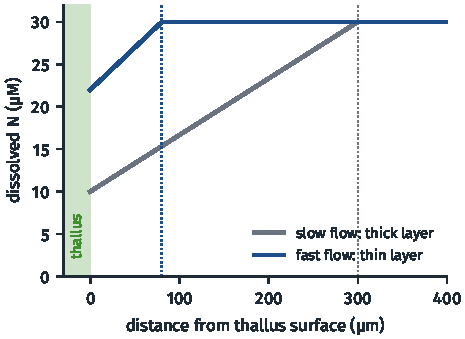
\includegraphics[width=\linewidth]{fig_bl_flow}
\fignote{Schematic profiles at the same uptake flux; $C_b$ bulk and $C_s$ surface concentration.}}
\end{frame}

% pos 43
\begin{frame}{Concentration gradient and diffusive supply}
\twocol{
\begin{itemize}
  \item High bulk [DIN]: large gradient, fast diffusive supply
  \item Low bulk [DIN]: small gradient, slow supply
  \item $C_s$ results from the balance of delivery and uptake
  \item In slow water, higher external concentration partly offsets a thick boundary layer
\end{itemize}}{
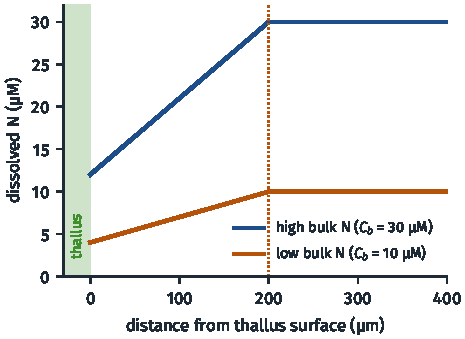
\includegraphics[width=\linewidth]{fig_bl_conc}
\fignote{Schematic profiles for the same layer thickness.}}
\end{frame}

% pos 44
\begin{frame}{Nutritional history}
\twocol{
\begin{itemize}
  \item Growth during low external N draws down internal reserves
  \item N-starved tissue may show fast \textit{initial} uptake after a pulse
  \item N-replete tissue takes up more slowly
  \item Possible causes: internal feedback, demand, changes in uptake machinery
  \item Depends on prior conditions and tissue health; the effect of starvation length varies
\end{itemize}}{
\begin{tikzpicture}[font=\scriptsize]
  \foreach \x/\lab/\w/\pts in {-1.7/{N-starved\\ fast initial uptake}/2.2/{(-0.3,0.35),(0.35,0.05),(-0.1,-0.4)}, 1.7/{N-replete\\ slower uptake}/0.8/{(-0.5,0.4),(-0.15,0.55),(0.2,0.55),(0.5,0.35),(-0.6,0.05),(-0.25,0.15),(0.1,0.2),(0.45,0.0),(-0.45,-0.3),(-0.1,-0.2),(0.25,-0.25),(0.55,-0.4),(-0.2,-0.6),(0.15,-0.6)}}{
    \fill[accent!35] (\x,0) circle (1.25);
    \fill[grey!20, draw=warm, very thick] (\x,0) circle (1.0);
    \begin{scope}[shift={(\x,0)}] \foreach \q in \pts {\node[font=\scriptsize] at \q {N};} \end{scope}
    \draw[-{Stealth}, sea, line width=\w pt] ($(\x,0)+(-1.9,-1.1)$) -- ($(\x,0)+(-0.85,-0.55)$);
    \node[align=center] at (\x,-1.85) {\lab};
  }
\end{tikzpicture}
\fignote{Schematic. Arrow width: relative uptake rate.}}
\end{frame}

% pos 45
\begin{frame}{Measuring uptake kinetics}
\twocol{
\begin{itemize}
  \item Uptake can be measured \textit{in situ} or under controlled laboratory conditions
  \item Usually from the \textbf{disappearance} of nutrient from the medium over a time interval after adding the alga
  \item Two designs: multiple flask (batch) and perturbation
  \item Depletion data give uptake rates, and from these the uptake kinetics
\end{itemize}}{
\begin{tikzpicture}[font=\scriptsize]
  \node[flow=sea, text width=4.6cm] (a) {flask: known volume, alga mass, temperature, light, starting [N]};
  \node[flow=accent, text width=4.6cm, below=0.35cm of a] (b) {sample the water over time};
  \node[flow=warm, text width=4.6cm, below=0.35cm of b] (c) {depletion curve: S against time};
  \node[flow=leaf, text width=4.6cm, below=0.35cm of c] (d) {uptake rate $V$ against S: kinetics};
  \draw[arr] (a) -- (b); \draw[arr] (b) -- (c); \draw[arr] (c) -- (d);
\end{tikzpicture}
\fignote{Detailed protocol: Lecture 9b.}}
\end{frame}
